\chapter{Successioni e serie di funzioni}
Il capitolo tratterà lo studio di successioni e serie di funzioni. I due argomenti sono tra loro collegati. Tuttavia, sebbene si possa ricondurre lo studio di una serie a quello di una successione, la successione delle ridotte n-esime, il capitolo non le porterà avanti in parallelo ma le analizzerà una per volta.
\section{Successioni di funzioni}
\begin{definition} \label{Def: Successione di funzioni}
     Si dice \textbf{successione di funzioni} l'insieme $\{\fn\}_{n \in \N}$ con
     \begin{equation}
         \fn: I \subseteq \R \to \R, n \in \N
     \end{equation}
\end{definition}
\begin{oss}
    Per questioni di praticità, laddove sia utilizzata una successione di funzioni, questa verrà indicata con $\fn$ anziché con $\{\fn\}_n\in \N$.
\end{oss}
Definito il concetto di successione di funzioni, si può iniziare a studiare la convergenza nelle sue diverse forme.\\
Si può innanzitutto notare che, fissato $\overline{x}\in I$, 
allora $\{\fn(\overline{x})\}_{n \in \N}$ è una successione numerica.
\begin{definition} \label{Def: Convergenza puntuale succ}
    Sia $\fn$ una successione di funzioni $I\to \R$. Allora si dice che $\fn$ \textbf{converge puntualmente} alla funzione $f: I \to \R$ se per ogni $\overline{x} \in I$ si ha che
    \begin{equation}
        \lim_{n \to +\infty} \fn(\overline{x}) = f(\overline{x})
    \end{equation}
    cioè
    \begin{equation}
        \forall\ \overline{x} \in I,\ \forall\ \varepsilon > 0,\ \exists\ N_{\varepsilon, x} \in \N\ \text{tale che}\ \forall\ n> N_{\varepsilon,x}\ \text{si ha}\ \left| \fn(x)-f(x)\right| < \varepsilon
    \end{equation}
    o, equivalentemente, sfruttando il criterio di Cauchy puntuale, se
\begin{equation}
    \forall\ x \in I, \forall\ \varepsilon > 0\ \exists\ N_{\varepsilon, x} \in N\ \text{tale che}\ \forall\ n,m > N_{\varepsilon, x}\ \text{si ha che}\ |\fn - f_m|<\varepsilon
\end{equation}
\end{definition}    
\begin{definition} \label{Def: Funzione limite}
    Inoltre, se c'è convergenza puntuale in $I$, è ben definita la \textbf{funzione limite} $f: I \to \R$ tale che
    \begin{equation}
        f(x) := \lim_{n \to +\infty} \fn(x)
    \end{equation}
\end{definition}
Occorre osservare che nel caso della convergenza puntuale, $N$ dipende e da $\varepsilon$ e da $x$, pertanto può essere utile dare una definizione più forte di convergenza che non dipenda da $x$.
\begin{definition} \label{Def: Convergenza uniforme succ}
    Si dice che $\fn$ \textbf{converge uniformemente} su $I$ a $f: I \to \R$ se
    \begin{equation}
        \forall\ \varepsilon>0\ \exists\ N_\varepsilon \in \N\ \text{tale che}\ \forall\ n>N_\varepsilon\ \text{si ha}\ \sup_{x \in I}|\fn(x)-f(x)| < \varepsilon
    \end{equation}
    cioè se
    \begin{equation}
    \lim_{n \to + \infty}{\sup_{x \in I} \left| \fn(x)-f(x)\right|}=0
    \end{equation}
    o, tramite il criterio di Cauchy uniforme,
    \begin{equation}
        \forall \ \varepsilon >0 \ \exists\ N_\varepsilon \in \N \ \text{tale che}\ \forall\ n,m > N_\varepsilon\ \text{si ha}\ \sup_{x \in I}{|\fn(x)-f_m(x)|}<\varepsilon
    \end{equation}
\end{definition}
\begin{figure}[H]
    Graficamente, la convergenza uniforme fa sì che si verifichi una situazione di questo tipo.
    \centering
        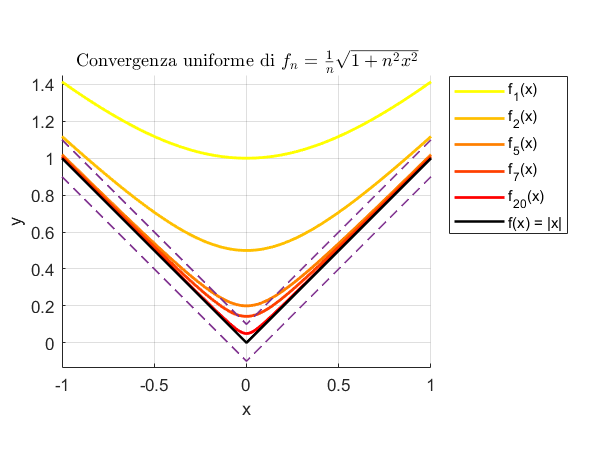
\includegraphics[width=0.4\textwidth]{Capitoli/Capitolo7/Convergenza uniforme.png}
\end{figure}
\begin{oss}
   Si può notare che la convergenza uniforme implica la convergenza puntuale, ma non è necessariamente vero il contrario.
    \end{oss}
\begin{oss}
 Dal punto di vista operativo, per stabilire l'uniforme convergenza di una successione di funzioni, si può agire in due modi:
    \begin{itemize}
       \item Calcolare $\sup\limits_{x \in I} |\fn(x)-f(x)|$ ricercando massimi e minimi con gli strumenti del calcolo in una variabile.
       \item Maggiorare opportunamente $\sup\limits_{x \in I} |\fn(x)-f(x)|$.
\end{itemize}
\end{oss}
\begin{example}
Si studi ora la convergenza della seguente successione di funzioni, il cui grafico è riportato in figura
\begin{equation*}
    \fn= x^n, \qquad x \in [0,1]
\end{equation*}
\begin{figure}[H]
    \centering
\begin{minipage}{0.6\textwidth}
Per quanto riguarda la convergenza puntuale si osserva che, fissato $x \in [0,1]$,
\begin{equation*}
    \lim_{n \to +\infty}{\fn(x)}= \lim_{n \to + \infty}= f(x) = \begin{cases}
        0 &\quad x \in [0,1]\\
        1 &\quad x=1
    \end{cases}
\end{equation*}
\end{minipage}
    \begin{minipage}{0.38\textwidth}
        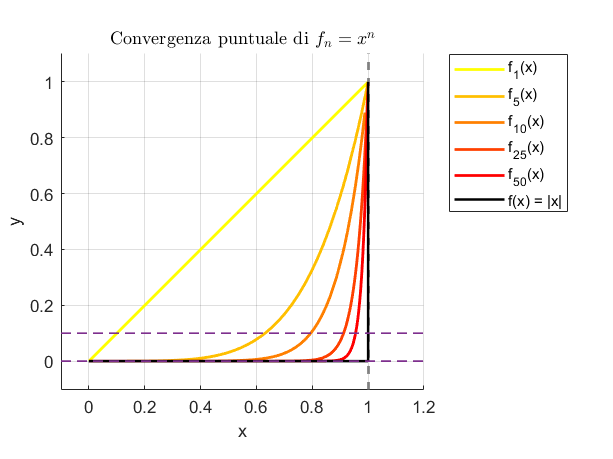
\includegraphics[width=\textwidth]{Capitoli/Capitolo7/Convergenza puntuale.png}
    \end{minipage}
    \end{figure}
Volendo poi studiare la convergenza uniforme, si ha che
\begin{equation*}
    \sup_{x \in [0,1]}{\left|\fn(x)-f(x)\right|} = \sup_{x \in [0,1]} \left\{ \sup_{x \in [0,1)} \left|\fn(x)-f(x)\right|, \left|\fn(x)-f(x)\right|\right\} = \sup_{x \in [0,1)}{\left|x^n-0\right|} = 1 \neq 0
\end{equation*}
Dunque in $[0,1]$ $\fn$ non converge in modo uniforme. D'altra parte è anche vero che la "patologia" si verifica in $x=1$, perciò valutando la convergenza uniforme in $[0,a],\ a < 1$, si ha che
\begin{equation*}
    \sup_{x \in [0,a]}{|\fn(x)-f(x)|}= x^n \big|_{[0,a]} = a^n \overset{n \to +\infty}{\to} 0
\end{equation*}
cioè $\fn$ uniformemente convergente a $0$ su ogni compatto $[0,a],\ a<1$.
\end{example}
\begin{theorem}[Scambio di limiti] \label{Teo: Scambio di limiti}
Sia $\fn: I \to \R$ tale che $\{\fn\}_n$ converge uniformemente in $I$ a $f: I \to \R$. Sia $x_0$ un punto di accumulazione per $I$ e si supponga che per ogni $n \in \N$ esista
\begin{equation}
    \ell_n:= \lim_{x \to x_0}{\fn(x)} \in \R
\end{equation}
Allora esistono i seguenti limiti e si ha
\begin{equation}
    \lim_{n \to +\infty}{\left(\lim_{x \to x_0} {\fn(x)}\right)}= \lim_{n \to +\infty}{\ell_n} = \lim_{x \to x_0} {f(x)} = \lim_{x \to x_0}{ \left( \lim_{n \to +\infty} {\fn(x)}\right)}
\end{equation}
\end{theorem}
\begin{proof}
    Si mostri che $\ell_n$ è una successione di Cauchy.\\
    Dalla convergenza uniforme delle $f_n$ si ha che
    \begin{equation}
        \forall\ \varepsilon>0\ \exists\ N_\varepsilon \in \N\ \text{tale che}\ \left| \fn(x)-f(x)\right|< \varepsilon,\ \forall\ x \in I
    \end{equation}
    Perciò, passando al limite per $x \to x_0$, si ha che
    \begin{equation}
        \left| \lim_{x \to x_0}{\fn(x)}-\lim_{x \to x_0}{f(x)}\right| = \left| \ell_n - \ell_m \right| \leq \varepsilon
    \end{equation}
    cioè $\ell_n$ è di Cauchy. Inoltre, $\{\ell_n\}_n$ è una successione di numeri reali, dunque essa deve convergere ad un qualche $\ell \in \R$. Ciò dimostra la prima metà della tesi.\\
    Rimane da provare che $f(x) \overset{x \to x_0}{\to} \ell$, cioè che $|f(x)-\ell| \to 0$. Dunque,
    \begin{equation}
    \begin{aligned}
        \left|f(x)-\ell\right| &= \left| f(x) - f_\nu(x)+ f_nu(x)- \ell_nu+ \ell_nu- \ell\right| =\\
        &=\overset{\text{Triang.}}{\leq} \left| f(x) - f_\nu(x) \right| +\left| f_\nu(x)- \ell_\nu(x)\right|+\left|\ell_\nu-\ell\right|
    \end{aligned}
    \end{equation}
    Si può notare che il primo termine è minore di $\varepsilon$ per ogni $\nu > N_\varepsilon$ per convergenza uniforme e che il terzo, essendo una successione numerica, è minore di $\varepsilon$ per un $\nu$ sufficientemente grande, poiché $\ell_n \to \ell$. Il secondo, fissato $\nu$ come sopra, soddisfa per ipotesi
    \begin{equation}
        \lim_{x \to x_0}{f_\nu(x)} = \ell_\nu
    \end{equation}
    Dunque, esiste un intorno $\U(x_0)$ tale che per ogni $ \in \U(x_0)$, $\left| f_\nu(x)- \ell_nu \right| < \varepsilon$.\\
    In conclusione, per $\nu$ fissato come sopra e $x \in \U(x_0)$ si ha che
    \begin{equation}
        \left|f(x)-\ell\right| < 3 \varepsilon
    \end{equation}
\end{proof}
\begin{oss}
    Il passaggio al limite nella prima parte della dimostrazione è consentito dal fatto che per ipotesi siano definite $\ell_n$ e $\ell_m$ reali.
\end{oss}
Da tale teorema discende come conseguenza immediata il seguente corollario
\begin{corollary}
    Sia $\fn$ una successione di funzioni continue uniformemente convergente in $I$ a $f:I \to \R$. Allora $f$ è continua. 
\end{corollary}
\begin{proof}
    Si mostri che preso $x_0$ punto di accumulazione per $I$, si ha
    \begin{equation}
        \lim_{x \to x_0}{f(x)}= f(x_0)
    \end{equation}
    Dunque sfruttando l'ipotesi di convergenza, si ha che
    \begin{equation}
        \lim_{x \to x_0}{\fn(x)}= \fn(x_0) \in \R
    \end{equation}
    D'altra parte vale lo scambio di limiti, quindi
    \begin{equation}
    \begin{aligned}
          f(x_0) &=  \lim_{n \to +\infty}{\fn(x_0)}= \lim_{n \to +\infty}{\left(\lim_{x \to x_0}{\fn(x)}\right)}=\\
          &= \lim_{x \to x_0}{ \left( \lim_{n \to +\infty}{\fn(x)}\right)}=\lim_{x \to x_0}{f(x)} 
    \end{aligned}
    \end{equation}
   
\end{proof}
Si mostrino ora due importanti risultati rispetto alla derivazione e all'integrazione di successioni di funzioni.
\begin{theorem} \label{Teo: Passaggio al limite sotto al segno di derivata}
    Sia $\{\fn\}_{n\in\N}$ una successione di funzioni $C^1[a,b]$. Sia la successione di numeri reali $\{\fn(x_0)\}_n$ convergente e sia $\{\fn'\}_n$ uniformemente convergente. Allora $\{\fn\}_n$ converge uniformemente in $[a,b]$ ad una funzione $f \in C^1([a,b])$ e 
    \begin{equation}
        \lim_{n \to +\infty}{\fn'(x)}= \left(\lim_{n \to +\infty}{\fn(x)}\right)'=f'(x)
    \end{equation}
\end{theorem}
\begin{theorem} \label{Teo: Passaggio al limite sotto al segno di integrale}
Sia $\{\fn\}_{n_\in \N}$ una successione di funzioni continue in $[a,b]$ uniformemente convergente in $[a,b]$ a $f$. Allora
\begin{equation}
    \lim_{n \to +\infty}{\int\limits_{a}^{b}{\fn(x)}\,dx}=\int\limits_{a}^{b}{\lim_{n \to +\infty}{\fn(x)}\,dx}= \int\limits_{a}^{b}{f(x)}\,dx
\end{equation}
\end{theorem}
\begin{example}
    In questo esempio si può osservare quanto sia rilevante l'ipotesi di uniforme convergenza della successione.
    \begin{figure}[H]
        \centering
        \begin{minipage}{0.5\textwidth}
            Si consideri la successione di funzioni data da 
            \begin{equation*}
            f_n(x)=\begin{cases}
            0 &\qquad x=0\\
            n & \qquad x \in (0, \frac{1}{n})\\
            0 &\qquad x \in (\frac{1}{n}, 1)\\
            \end{cases}
            \end{equation*}
            e si osservi che
            \begin{equation*}
                \int\limits_{0}^{1}{\fn(x)}\,dx=1 \neq \int\limits_{0}^{1}{f(x)}\,dx = 0
            \end{equation*}
        \end{minipage}
        \begin{minipage}{0.4\textwidth}
        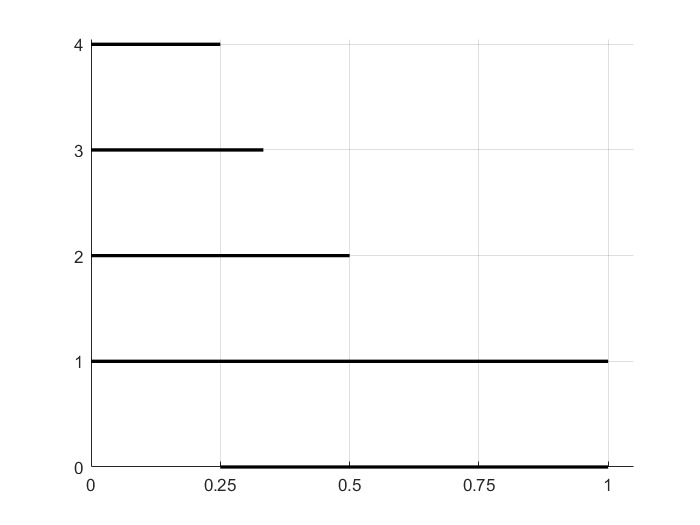
\includegraphics[width=\textwidth]{Capitoli/Capitolo7/Esempio integrale succ. funz..png}
        \end{minipage}
    \end{figure}
    poiché non uniformemente convergente.
\end{example}
\section{Serie di funzioni}
Come già accennato all'inizio del capitolo, quando si parla di serie, ci si può in realtà rifare alle successioni. Perciò in questa sezione verranno rielaborate le informazioni del capitolo precedente adattandole alle serie di funzioni.
\begin{definition}
    Sia $\{\fn\}_{n \in \N}$ una successione di funzioni, $\fn: I \subseteq \R \to \R$. Si dice \textbf{serie di funzioni} di termine generale $\fn$ la successione di funzioni delle somme parziali di $\{\fn\}_{n \in \N}$ data da
    \begin{equation}
        \sn(x)=\sum\limits_{n=1}^{N}{\fn(x)}
    \end{equation}
\end{definition}
Si passi alla convergenza.
\begin{definition}
    Sia $\sum\limits_{n=1}^{\infty}{\fn(x)}$ una serie di funzioni. Allora si dice che la serie \textbf{converge puntualmente} in I se la successione $\{\sn\}_{n \in \N}$ converge puntualmente in I. In maniera equivalente, la serie converge se, detta
    \begin{equation}
        s(x)=\lim_{n \to +\infty}{\sn(x)}
    \end{equation}
    si ha che
    \begin{equation}
        \forall\ x \in I,\ \forall\ \varepsilon>0,\ \exists\ N_{\varepsilon, x}\ \text{tale che}\ \forall N>N_{\varepsilon, x}\ \text{si ha che}\ |\sn(x)-s(x)|< \varepsilon
    \end{equation}
    o, ancora, sfruttando il criterio di Cauchy, se
    \begin{equation}
        \forall\ x \in I,\ \forall\ \varepsilon>0,\ \exists\ N_{\varepsilon, x}\ \text{tale che}\ \forall\ n>N_{\varepsilon, x},\ \forall p \in \N\ \text{si ha}\ |f_{n+1}(x)+ \dots+ f_{n+p}(x)|<\varepsilon
    \end{equation}
\end{definition}
\begin{definition}
    Se la serie converge puntualmente è ben definita la funzione \textbf{somma}
    \begin{equation}
        s(x)=\lim_{n \to +\infty}{\sn(x)}= \sum_{n=0}^{\infty}{\fn(x)}
    \end{equation}
\end{definition}
\begin{definition}
Sia $\sum\limits_{n=1}^{\infty}{\fn(x)}$ una serie di funzioni. Allora si dice che la serie \textbf{converge uniformemente} in I se la successione $\{\sn\}_{n \in \N}$ converge uniformemente in I. In maniera equivalente, sfruttando il criterio di Cauchy uniforme, se
\begin{equation}
\forall\ \varepsilon>0\ \exists\ N_\varepsilon \in \N\ \text{tale che}\ \forall\ n > N_\varepsilon\ \forall\ p \in \N\ \text{si ha}\ \sup_{x \in I}{|f_{n+1}(x)+\dots+f_{n+p}(x)|}<\varepsilon 
\end{equation}
\end{definition}
Verranno introdotte ora due nuove nozioni di convergenza proprie delle serie di funzioni.
\begin{definition}
    Sia $\{\sn\}_{n \in \N}$ una serie di funzioni. Si dice che la serie \textbf{converge assolutamente}  se
    \begin{equation}
        \sum_{n}{|\fn(x)|}
    \end{equation}
    converge per ogni $x \in I$
\end{definition}
In particolare si può osservare che, da una parte, la convergenza assoluta implica la convergenza puntuale, dall'altra, convergenza uniforme e assoluta non si implicano in nessuna direzione.
\begin{example}
    Si mostri inoltre con un esempio che la convergenza puntuale non implica la convergenza assoluta. Sia
    \begin{equation*}
        \fn(x)=\frac{(-1)^n}{n}
    \end{equation*}
    Allora $\sum\limits_{n}{\fn}$ converge ma $\sum\limits_{n}{|\fn|}$ diverge.
\end{example}
\begin{definition}
    Sia $\sum\limits_{n=1}^{\infty}{\fn(x)}$ una serie di funzioni. Si dice che essa converge totalmente in $I$ se esiste una successione numerica $\{k_n\}_n$ con $k_n>0$ per ogni $n$ tale che
    \begin{enumerate}
        \item $|\fn|<k_n$
        \item $\sum\limits_{n}{k_n}$ converge
    \end{enumerate}
\end{definition}
In particolare si può osservare che la convergenza totale implica la convergenza assoluta (e quindi anche quella puntuale). Segue la dimostrazione di tale fatto.
\begin{proof}
    Se $\sum\limits_{n}\fn$ converge totalmente, allora per definizione esiste una successione $k_n$ tale che $|\fn|<k_n$ e tale che la propria serie converga. Ma allora si ha che
    \begin{equation}
        \sum_{n}{|\fn|} < \sum_{n}{k_n}= \ell \in \R
    \end{equation}
    Perciò, per il teorema del confronto per le serie, $\sum\limits{|\fn|}$ converge e, quindi, $\sum\limits{\fn}$ converge assolutamente.
\end{proof}
\begin{theorem}[Criterio di Weierstrass] \label{Teo: Criterio di Weierstrass (convergenza totale)}
Una serie di funzioni $\sum\limits_{n=1}^{\infty}{\fn(x)}$ totalmente convergente in $I$ è ivi uniformemente convergente.
\end{theorem}
\begin{proof}
    Si sfrutti il criterio di Cauchy uniforme per le serie. L'obiettivo quindi è mostrare che esista un $N_\varepsilon$ tale che $|f_{n+1}+ \dots+ f_{n+p}|< \varepsilon,\ \forall\ n > N_\varepsilon,\ \forall\ P\in \N$.
    Dunque, si fissi $\varepsilon>0$. Per ipotesi di convergenza totale si ha che $\sum\limits_{n=1}^{\infty}{k_n}$ converge, perciò esiste un $N_\varepsilon>0$ tale che per ogni $n>N_\varepsilon$ si ha che $|k_{n+1}+\dots+k_{n+p}|< \varepsilon\ \forall\ p \in \N$. 
    Tuttavia, $k_n>0\ \forall n$, quindi si può togliere il modulo. D'altra parte, $|\fn|<k_n$ e, di conseguenza, a patto di prendere $n> N_\varepsilon$ si ha che, $\forall\ p \in \N,\ \forall x \in I$, vale
    \begin{equation}
    \begin{aligned}
        |f_{n+1}(x)+ \dots + f_{n+p}(x)| &\leq |f_{n+1}(x)|+ \dots + |f_{n+p}(x)|<\\ 
        &< k_{n+1}+ \dots + k_{n+p} < \varepsilon
    \end{aligned}
    \end{equation}
    Dunque è verificato il criterio di Cauchy uniforme e la serie converge uniformemente in I.
\end{proof}
\begin{oss}
    Il teorema offre una condizione sufficiente per la convergenza uniforme delle serie di funzioni.
\end{oss}
Infine, si enuncino i teoremi sulla continuità della somma e su derivazione e integrazione di serie di funzioni.
\begin{theorem}
    Siano $I \subseteq \R,\ \fn \in C^0(I)$ e sia $\sum\limits_{n=0}^{\infty}{\fn(x)}$ uniformemente convergente in $I$ a $s$. Allora la funzione somma $s(x)$ è continua in $I$.
\end{theorem}
\begin{theorem}
    Sia $\fn \in C^1([a,b])$ e si supponga $\sum\limits_{n=0}^{\infty}{\fn(x)}$ puntualmente convergente in $[a,b]$ a $s(x)$ e $\sum\limits_{n=0}^{\infty}{\fn'(x)}$ uniformemente convergente in $[a,b]$. Allora
    \begin{equation}
        \sum\limits_{n=0}^{\infty}{\fn'(x)}= 
        \left(\sum\limits_{n=0}^{\infty}{\fn(x)}\right)'= s'(x) \qquad \forall\ x \in [a,b]
    \end{equation}
\end{theorem}
\begin{theorem}
    Sia $\fn \in C^0([a,b])$ e sia $\sum\limits_{n=0}^{\infty}{\fn(x)}$ uniformemente convergente in $[a,b]$ a $s$. Allora
    \begin{equation}
        \sum\limits_{n=0}^{\infty}{\int\limits_{a}^{b}{\fn(x)}\, dx}= \int\limits_{a}^{b}{\sum\limits_{n=0}^{\infty}{\fn(x)}\, dx}= \int\limits_{a}^{b}{s(x)}\, dx
    \end{equation}
\end{theorem}
\section{Serie di potenze}
\begin{definition}
Si dice \textbf{serie di potenze} reale di centro $x_0 \in \R$ una serie di funzioni della forma
\begin{equation}
    a_0+ \sum_{n=1}^{\infty}{a_n(x-x_0)^n} \qquad a_n \in \R\ \forall\ n=0,1,\dots
\end{equation}
\end{definition}
\begin{oss}
    Mediante opportune traslazioni è possibile passare da una serie di potenze centrata in $x_0$ a una centrata in $0$ della forma
    \begin{equation}
        \sum_{n=0}^{\infty}{a_n x^n}
    \end{equation}
\end{oss}
\begin{definition}
    Si dice \textbf{raggio di convergenza} della serie $\sum\limits_{n=0}^{\infty}{a_n x^n}$ l'estremo superiore $R$ dell'insieme $E$ dei numeri reali $\xi$ nei quali la serie converge, ossia
    \begin{equation}
        R= \sup E \qquad E=\left\{ \xi \in \R \mid \sum_{n=0}^{\infty}{a_n x^n}\ \text{converge}\right\}
    \end{equation}
\end{definition}
La caratterizzazione di $R$ si ha a partire dal seguente teorema.
\begin{theorem} \label{Teo: Caratterizzazione del raggio di convergenza}
    Sia $R$ raggio di convergenza della serie di potenze. Se $R=0$, allora la serie converge solo in $0$. Se $R>0$, la serie converge totalmente in ogni $[a,b] \subset (-R, R)$ e non converge per $|x|>R$.
\end{theorem}
\begin{proof}
 Si mostri che se $\sum\limits_{n=0}^{\infty}{a_n \xi^n}$ converge per un qualche $\xi \neq 0$ allora converge totalmente in ogni intervallo $[-\eta, \eta] \subset (|-\xi|, |\xi)$.\\
 Per ipotesi di convergenza della serie, $|a_n \xi^n|$ deve essere una successione infinitesima (e perciò limitata) per $n\to \infty$, ovvero
 \begin{equation}
     \exists\ M>0\ \text{tale che}\ |a_n||\xi|^n\leq M
 \end{equation}
 A questo punto, fissato $\eta>0$ tale che $\eta<|\xi|$, si calcoli il termine generale della serie per un qualche $x \in [-\eta, \eta]$.
 \begin{equation}
     |a_n x^n| = \left|a_n x^n \frac{\xi^n}{\xi^n}\right|=\left|a_n \xi^n\right| \left|\frac{x}{\xi}\right|^n \leq M \left(\frac{|x|^n}{\left|\xi\right|^n} \right)\leq M \left(\frac{\eta}{\left| \xi \right|} \right)^n =k_n
 \end{equation}
 Poiché $k_n$ è il termine generale di una serie geometrica di ragione $\left(\tfrac{\eta}{\left| \xi \right|} \right)^n < 1$, essa è convergente. Quindi
 \begin{equation}
 \forall\ x \in [-\eta, \eta],\ \sum\limits_{n=0}^{\infty}{|a_n \xi^n|} \leq M \sum_{n=0}^{\infty}{\left(\frac{\eta}{\left| \xi \right|} \right)^n}
 \end{equation}
 che soddisfa le condizioni di convergenza totale con $k_n=\left(\tfrac{\eta}{\left| \xi \right|} \right)^n$.\\
 Nel caso in cui $R=0$, per quanto detto, la serie non può convergere in punti $\xi$ tali che $\xi \neq 0$.\\
 Nel caso in cui $|x|>R$, si ha che, per $x>R$ la serie non converge perché andrebbe in contraddizione con la definizione di $\sup$ propria di $R$; discorso analogo vale per $x<-R$, siccome la convergenza in tale punto implicherebbe la convergenza in ogni $[-\eta, \eta] \subset (-|x|, |x|)$ e, se così fosse, si contraddirebbe nuovamente la definizione di $\sup$.
\end{proof}
\begin{oss}
Il teorema dà un'ulteriore informazione: se $R= +\infty$, allora la serie di potenze converge totalmente in ogni compatto di $\R$.
\end{oss}
\begin{theorem}[Criterio di Cauchy-Hadamard] \label{Teo: Criterio di Cauchy-Hadamard}
Sia $\sum\limits_{n=0}^{\infty}{a_n x^n}$ una serie di potenze. Se esiste il limite
\begin{equation}
    \ell=\lim_{n \to \infty}{\sqrt[n]{|a_n|}}
\end{equation}
    allora il raggio di convergenza vale
    \begin{equation}
        R = \begin{cases}
            +\infty &\qquad \ell=0\\
            \frac{1}{\ell} &\qquad \ell \neq 0\\
            0 &\qquad \ell = \infty
        \end{cases}
    \end{equation}
\end{theorem}
\begin{proof}
    Per ogni $x \neq 0$ risulta
    \begin{equation}
        \lim_{n \to \infty}{\sqrt[n]{|a_n x^n|}} = \ell|x| := L
    \end{equation}
    Allora, dallo studio di $l$ si ha che
    \begin{enumerate}
        \item $\ell=0 \Rightarrow L=0$, perciò, per criterio della radice delle serie numeriche, la serie converge assolutamente per ogni $x \neq 0$. Inoltre, poiché la serie converge anche con $x=0$, $R=+\infty$.
        \item $\ell= \infty \Rightarrow L = \infty$, quindi, per ogni $x \neq 0$ la serie non converge assolutamente, cioè $R=0$.
        \item $0< \ell<\infty$, per il criterio della radice delle serie numeriche, quando $L<1 \iff |x|< \tfrac{1}{\ell}$ la serie converge assolutamente. Invece, quando $L>1 \iff |x|>\tfrac{1}{\ell}$ la serie non converge assolutamente, quindi, $R= \tfrac{1}{\ell}$.
    \end{enumerate}
\end{proof}
Oltre al criterio della radice, vale anche il criterio del rapporto, di cui viene dato solo l'enunciato, dal momento che la sua dimostrazione è analoga a quella precedente con l'eccezione di applicare il criterio del rapporto per le serie numeriche anziché quello della radice.
\begin{theorem}[Criterio di d'Alembert]
    Sia $\sum\limits_{n=0}^{\infty}{a_n x^n}$ una serie di potenze. Se esiste il limite
    \begin{equation}
        \ell= \lim_{n \to \infty}{\frac{a_{n+1}}{a_n}}
    \end{equation}
    allora il raggio di convergenza della serie vale
    \begin{equation}
        R= \begin{cases}
        +\infty &\qquad \ell=0\\
        \frac{1}{\ell} &\qquad \ell \neq 0\\
        0 &\qquad \ell = \infty
        \end{cases}
    \end{equation}
\end{theorem}
\begin{example}
    RECUPERARE ESEMPIO E PARTE SUL TEOREMA DI ABEL
\end{example}
\subsection{Sviluppabilità di una funzione in serie di potenze}
\begin{theorem}[Derivazione di serie di potenze] \label{Teo: Derivazione di serie di potenze}
Sia $\sum\limits_{n=0}^{\infty}{a_n x^n}$ una serie di potenze con raggio di convergenza $R>0$. Sia poi $f$ la sua funzione somma. Allora la serie
\begin{equation}
    \sum\limits_{n=1}^{\infty}{\left(a_n x^n\right)'}= \sum\limits_{n=1}^{\infty}{n a_n x^{n-1}}= \sum\limits_{j=0}^{\infty}{\left(j+1\right)a_{j+1} x^j}
\end{equation}
ha lo stesso raggio di convergenza $R$. Inoltre, esiste $f'(x)\ \forall\ x \in (-R, R)$ e
\begin{equation}
    f'(x)=\sum\limits_{n=0}^{\infty}{\left(n+1\right)a_{n+1} x^n}
\end{equation}
\end{theorem}
\begin{proof}
    Per semplicità si supponga che esista e valga 
    \begin{equation}
        \lim_{n \to \infty}{\sqrt[n]{|a_n|}}=\frac{1}{R}
    \end{equation}
    e si calcoli il raggio di convergenza della serie derivata. Allora
    \begin{equation}
        \lim_{j \to + \infty}{\sqrt[j]{(j+1)|a_{j+1}|}} = \lim_{j \to + \infty}{\sqrt[j]{(j+1)}} \lim_{j \to + \infty}{\sqrt[j]{|a_{j+1}|}}= \lim_{j \to + \infty}{{\left(|a_{j+1}|^{\frac{1}{j+1}}\right)^{\frac{j+1}{j}}}}  \overset{\ref{Teo: Criterio di Cauchy-Hadamard}}{=} \frac{1}{R}
    \end{equation}
    E quindi, ponendosi in un compatto $[a,b] \subset (-R, R)$ in cui la serie derivata e la serie di potenze convergono totalmente e applicando il teorema, si ha la tesi.
\end{proof}
Reiterando tale procedimento, si può osservare che la somma della serie di potenze deve essere di classe $C^\infty$. Dunque, si può stabilire una condizione necessaria di buona approssimazione di una funzione $f$ tramite una serie di potenze, cioè il fatto che $f \in C^{\infty}$. Tale questione non si pone invece parlando di serie di Fourier.\\
D'altro canto, si possono introdurre ora le serie di Taylor. 
\begin{proposition}
Sia $x_0=0$ e sia $f \in C^\infty$ tale che in $(-R, R)$ si abbia
\begin{equation}
    f(x)= \sum\limits_{n=0}^{\infty}{a_n x^n}
\end{equation}
Allora tale serie è la serie di Taylor di $f$.
\end{proposition}
\begin{proof}
Per quanto detto nel teorema precedente, deve valere
\begin{equation}
    f^{(m)}(x)= \sum\limits_{n=m}^{\infty}{\frac{n!}{(n-m)!} a_n x^{n-m}}
\end{equation}
e quindi, ponendo $x=0$, tutti gli addendi dopo il primo si azzerano, lasciando così
\begin{equation}
    f^{(m)}(0)=a_n m! \Rightarrow a_n=\frac{f^{(m)}}{m!} \qquad \forall\ n
\end{equation}
cioè $a_n$ è il coefficiente di Taylor.
\end{proof}
\begin{definition} \label{Def: Funzione analitica}
    Si dice che una funzione $f$ è una funzione \textbf{analitica} in $\U(0)$ se sull'intervallo $(-\varrho, \varrho)$ si ha che
    \begin{equation}
        f(x)= \sum\limits_{n=0}^{\infty}{a_n x^n}
    \end{equation}
\end{definition}
\begin{oss}
    Esistono funzioni di classe $C^\infty$ la cui serie di Taylor abbia raggio di convergenza $R=0$.
\end{oss}
\begin{oss}
    La definizione di funzione analitica può essere formulata in un generico $\U(x_0)$ e si può dimostrare che se $f$ è analitica in $(x_0-\varrho, x_0+\varrho)$, allora lo è anche in un intorno di ogni $x_1 \in (x_0-\varrho, x_0+\varrho)$.
\end{oss}
\begin{theorem}
    Le funzioni analitiche sono un sottoinsieme proprio di $C^\infty$
\end{theorem}
\begin{proof}
 Si dimostri il teorema con un controesempio. Sia 
 \begin{equation}
     f(x)= \begin{cases}
         e^{-\frac{1}{x^2}} &\qquad x \neq 0\\
         0 &\qquad x=0
     \end{cases}
 \end{equation}
 Tale funzione è continua in $\R$ e verifica 
 \begin{equation}
     \lim_{x \to 0}{f(x)}=0= \lim_{x \to 0}{ e ^{-\frac{1}{x^2}}}
 \end{equation}
 Allora, calcolandone la derivata prima si ha 
 \begin{equation}
     f'(x)= \begin{cases}
         \frac{2}{x^3} e^{-\tfrac{1}{x^2}} & \qquad x \neq 0\\
         \lim\limits_{x \to 0}{\frac{f(x)-f(0)}{x}}= \lim\limits_{x \to 0}{\frac{e^{-\frac{1}{x^2}}}{x}}=0 &\qquad x=0
     \end{cases}
 \end{equation}
 Continuando a derivare, si ottiene sempre un'equazione del tipo
 \begin{equation}
     f^{(m)}(x)=\begin{cases}
         C e^{-\frac{1}{x^2}} &\qquad x\neq0\\
         0 &\qquad x=0
     \end{cases}
 \end{equation}
 cioè, $f \in C^\infty(\R)$. Tuttavia, $f^{(m)}(0)=0$. Pertanto la serie di Taylor dovrebbe essere la funzione nulla, ma $f \not\equiv 0\ \forall\ \dot{\U}(0)$, quindi non è analitica.
\end{proof}
Allora, per terminare, si dia ora un criterio per stabilire se una funzione sia sviluppabile come serie di potenze.
\begin{theorem}[Criterio di sviluppabilità] \label{Teo: Criterio di sviluppabilità}
    Sia $f \in C^\infty(-\varrho, \varrho)$ per un qualche $\varrho>0$. Sia poi
    \begin{equation}
        \sup_{x \in (-\varrho, \varrho)}{|f^{n}(x)|}\leq L^{n+1}n!
    \end{equation}
    per un'opportuna costante $L>0$. Allora $f$ è analitica in un intorno $\U(0)$
\end{theorem}
\begin{oss}
    Funzioni come $e^x,\ \sin(x), \ \cos(x)$ sono analitiche.
\end{oss}
%\section{Spazi metrici}